\begin{figure}[!h]
\caption{Routine pc use $\times$ routine index by job type (continuous)}
\subfloat[Below GCSE C]{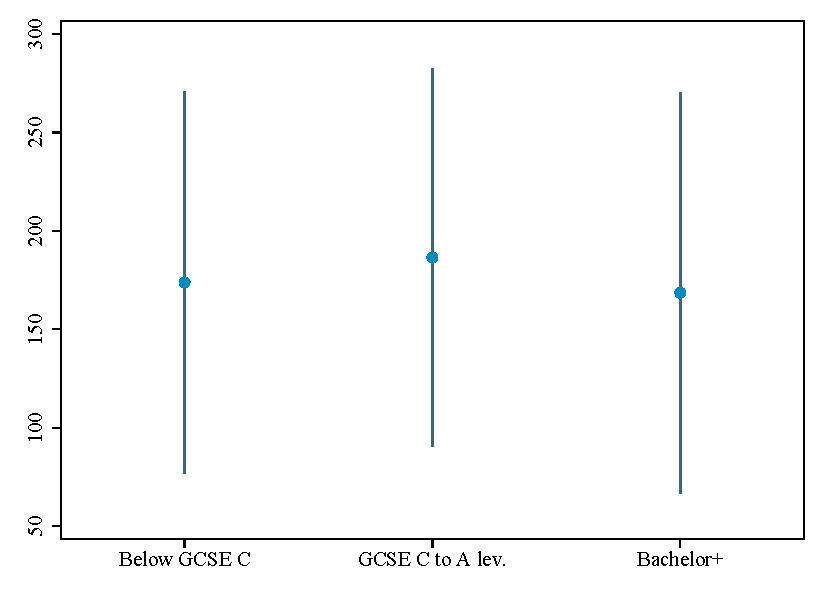
\includegraphics[width=.5\textwidth]{../output/routineContInt1}} \subfloat[GCSE C-A levels]{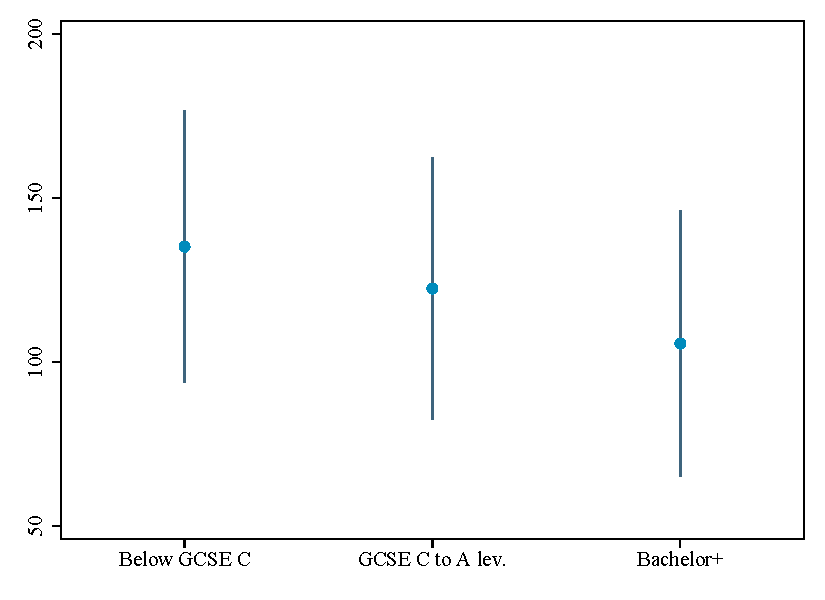
\includegraphics[width=.5\textwidth]{../output/routineContInt2}} \\ \subfloat[Bachelor+]{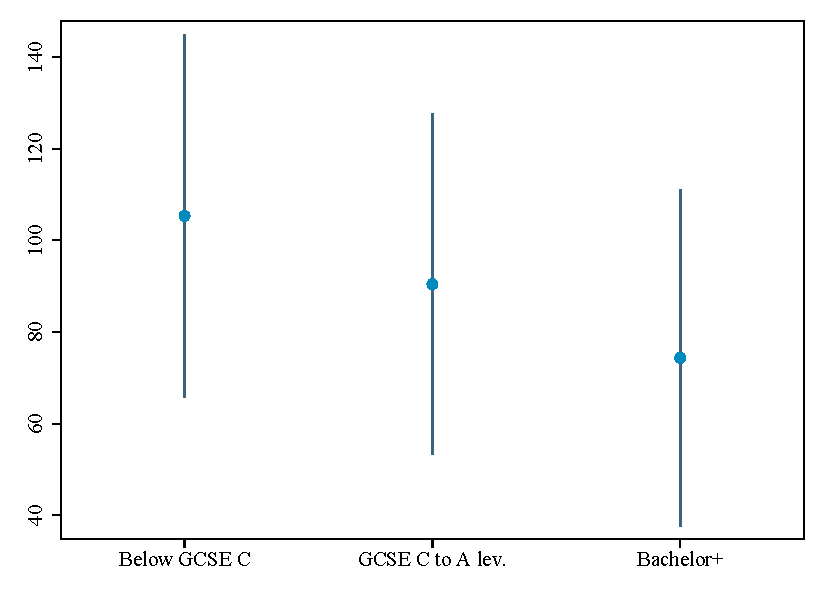
\includegraphics[width=.5\textwidth]{../output/routineContInt3}} \subfloat[Below GCSE C/GCSE C-A levels]{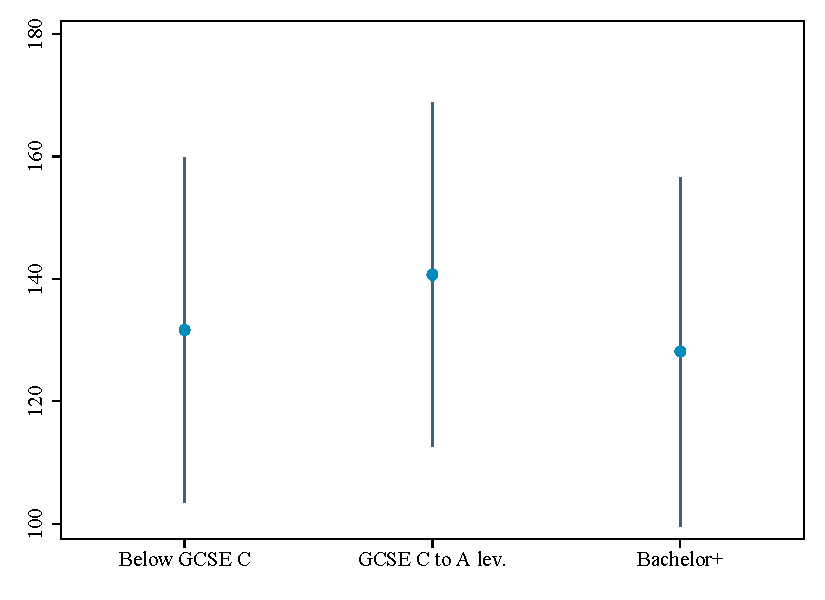
\includegraphics[width=.5\textwidth]{../output/routineContInt12}} \\ \subfloat[GCSE C-A levels/Bachelor+]{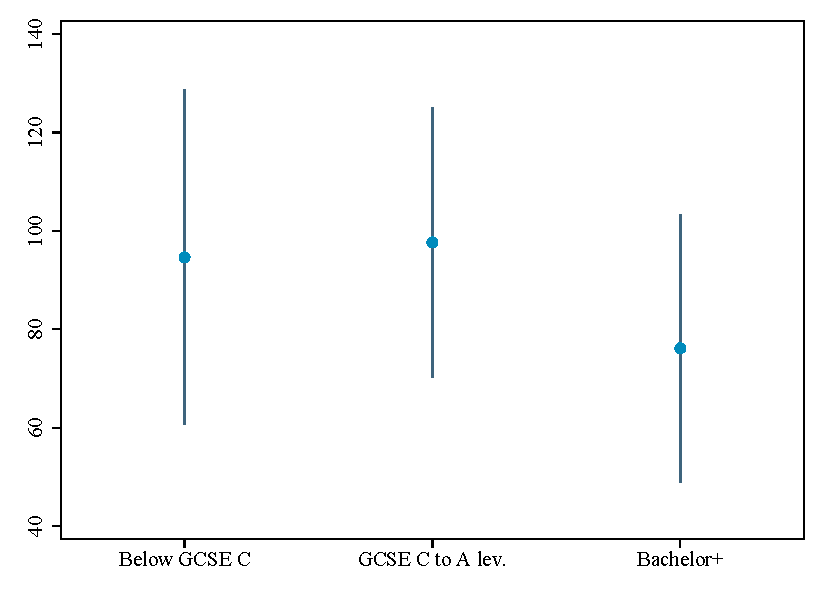
\includegraphics[width=.5\textwidth]{../output/routineContInt23}} 
\par \begin{minipage}[h]{\textwidth}{\scriptsize\textbf{Note:} graphs show regression coefficients. Regressions include occupation and year fixed effects. CI based on robust standard errors. Higher values indicate less complex pc use. I assign a value of 1 to people who do not use a computer. Table generated on 28 Apr 2020 at 19:00:17.}\end{minipage}
\end{figure}
